\documentclass[nooutcomes]{ximera}
%\documentclass[space,handout,nooutcomes]{ximera}

% For preamble materials

\usepackage{pgf,tikz}
\usepackage{mathrsfs}
\usetikzlibrary{arrows}
\usepackage{framed}
\usepackage{amsmath}
\pgfplotsset{compat=1.17}

\def\fixnote#1{\begin{framed}{\textcolor{red}{Fix note: #1}}\end{framed}}  % Allows insertion of red notes about needed edits
%\def\fixnote#1{}

\def\detail#1{{\textcolor{blue}{Detail: #1}}}   

\pdfOnly{\renewenvironment{image}[1][]{\begin{center}}{\end{center}}}

\graphicspath{
  {./}
  {chapter1/}
  {chapter2/}
  {chapter4/}
  {proofs/}
  {graphics/}
  {../graphics/}
}

\newenvironment{sectionOutcomes}{}{}


%%% This set of code is all of our user defined commands
\newcommand{\bysame}{\mbox{\rule{3em}{.4pt}}\,}
\newcommand{\N}{\mathbb N}
\newcommand{\C}{\mathbb C}
\newcommand{\W}{\mathbb W}
\newcommand{\Z}{\mathbb Z}
\newcommand{\Q}{\mathbb Q}
\newcommand{\R}{\mathbb R}
\newcommand{\A}{\mathbb A}
\newcommand{\D}{\mathcal D}
\newcommand{\F}{\mathcal F}
\newcommand{\ph}{\varphi}
\newcommand{\ep}{\varepsilon}
\newcommand{\aph}{\alpha}
\newcommand{\QM}{\begin{center}{\huge\textbf{?}}\end{center}}

\renewcommand{\le}{\leqslant}
\renewcommand{\ge}{\geqslant}
\renewcommand{\a}{\wedge}
\renewcommand{\v}{\vee}
\renewcommand{\l}{\ell}
\newcommand{\mat}{\mathsf}
\renewcommand{\vec}{\mathbf}
\renewcommand{\subset}{\subseteq}
\renewcommand{\supset}{\supseteq}
%\renewcommand{\emptyset}{\varnothing}
%\newcommand{\xto}{\xrightarrow}
%\renewcommand{\qedsymbol}{$\blacksquare$}
%\newcommand{\bibname}{References and Further Reading}
%\renewcommand{\bar}{\protect\overline}
%\renewcommand{\hat}{\protect\widehat}
%\renewcommand{\tilde}{\widetilde}
%\newcommand{\tri}{\triangle}
%\newcommand{\minipad}{\vspace{1ex}}
%\newcommand{\leftexp}[2]{{\vphantom{#2}}^{#1}{#2}}

%% More user defined commands
\renewcommand{\epsilon}{\varepsilon}
\renewcommand{\theta}{\vartheta} %% only for kmath
\renewcommand{\l}{\ell}
\renewcommand{\d}{\, d}
\newcommand{\ddx}{\frac{d}{dx}}
\newcommand{\dydx}{\frac{dy}{dx}}


\usepackage{bigstrut}


\title{Constructions Problems}
\author{Bart Snapp and Brad Findell}
\begin{document}
\begin{abstract}
Short-answer problems about constructions. 
\end{abstract}
\maketitle

\begin{question}
What is your name?
\begin{freeResponse}
\end{freeResponse}
\end{question}


% What are the rules for compass and straightedge constructions?
% What is a collapsing compass? Why don't we use them or worry about them any more?
% Prove that the collapsing compass is equivalent to the modern compass.
%
%\begin{hint}[Transferring a Segment]\index{compass and straightedge!transferring a segment}
%Given a segment, we wish to move it so that it starts on a given
%point, on a given line.
%\begin{enumerate}        
%\item Draw a line through the point in question.
%\item Open your compass to the length of the line segment and draw a circle with the given point as its center.
%\item The line segment consisting of the given point and the intersection of the circle and the line 
%is the transferred segment.
%\end{enumerate}
%\end{hint}



\begin{problem}
Given a line segment, construct an equilateral triangle whose edge has the length of the given segment. Explain the steps in your construction and how you know it works.
\begin{freeResponse}
\begin{hint}%[Equilateral Triangle]\index{compass and straightedge!equilateral triangle} 
%We wish to construct an equilateral triangle given the length of one side.
\begin{enumerate} 
%\item Open your compass to the width of the line segment.
\item Draw two circles, one with each end point as the center and with the other as a point on the circle. 
\item The circles intersect at two points.  Choose one and 
connect it to both of the line segment's endpoints.
\end{enumerate}
\begin{image}
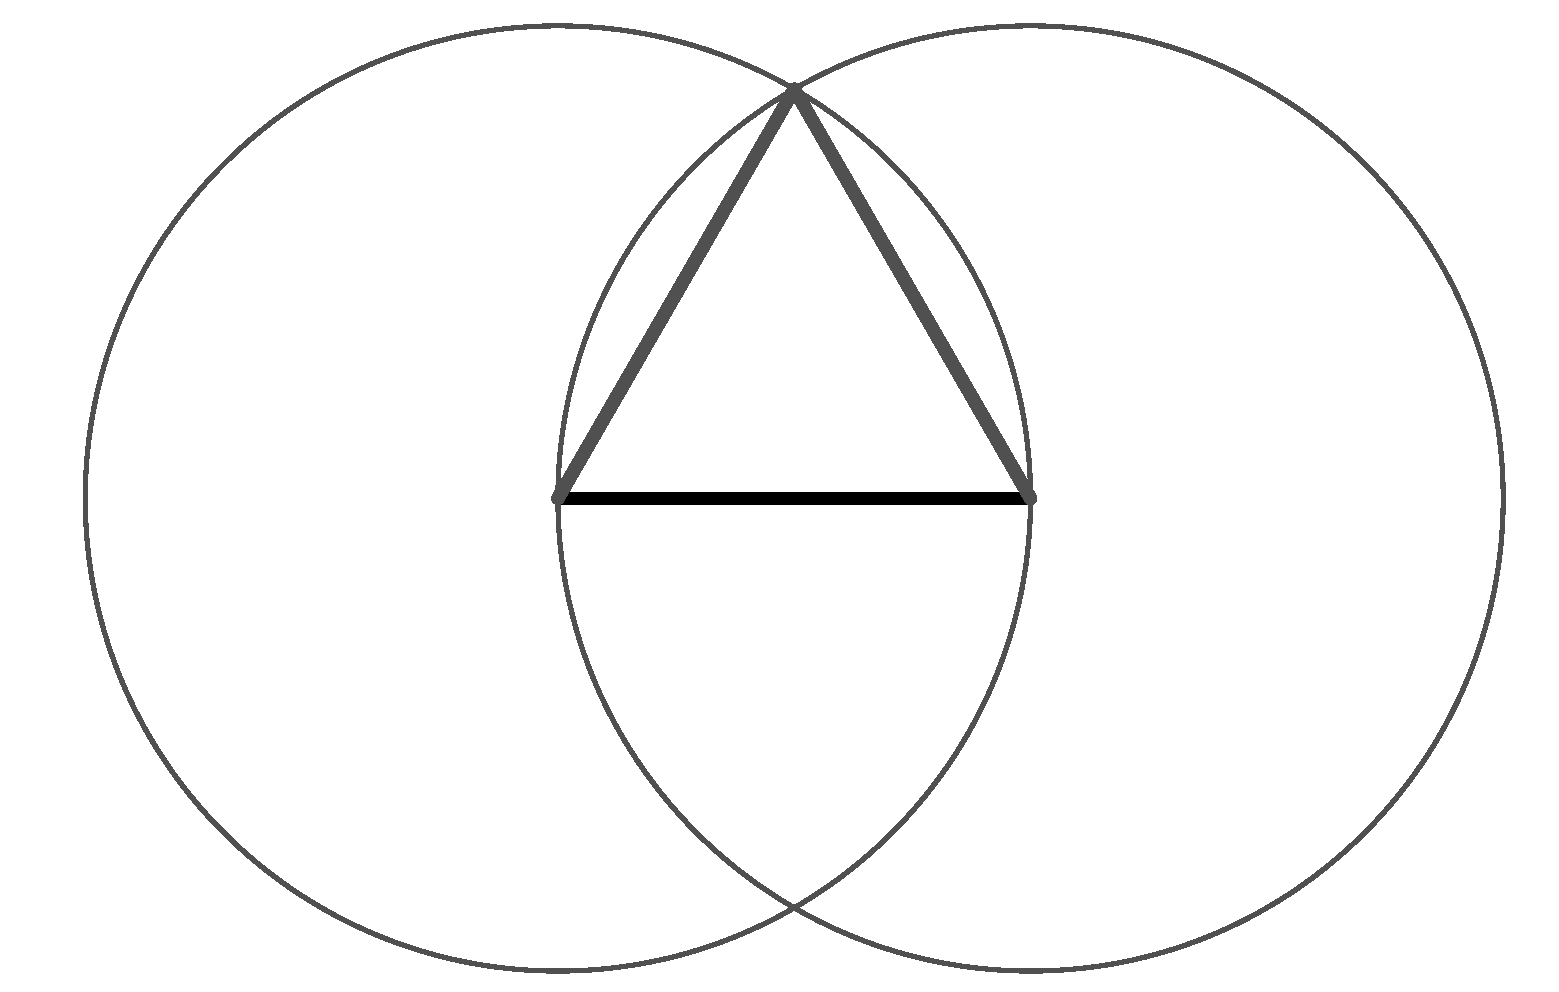
\includegraphics{eqtri.png}
\end{image}
\end{hint}
\end{freeResponse}
\end{problem}

\begin{problem}
Use a compass and straightedge to bisect a given line segment. Explain the steps in your construction and how you know it works.
\begin{freeResponse}
\begin{hint}%[Bisecting a Segment]\index{compass and straightedge!bisecting a segment} 
%Given a segment, we wish to cut it in half.
\begin{enumerate}
%\item Open your compass to the width of the segment.
\item Draw two circles, one with each end point as the center and with the other as a point on the circle. 
\item The circles intersect at two points.  Draw a line through 
these two points.
\item The new line bisects the original line segment.
\end{enumerate}
\begin{image}
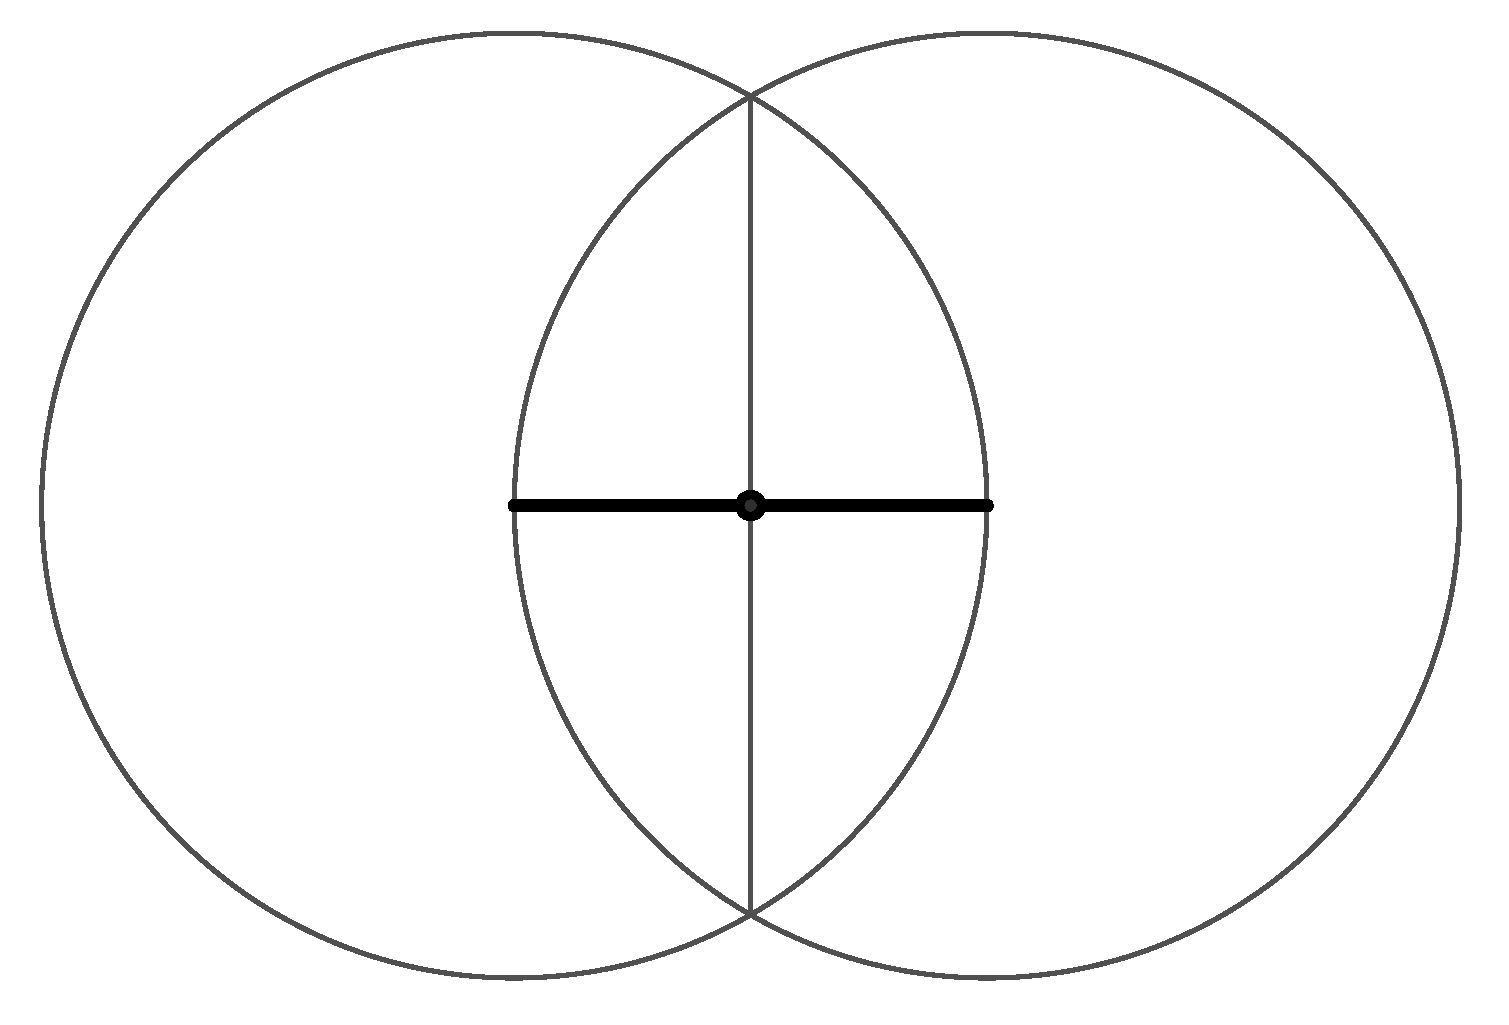
\includegraphics{bisectseg.png}
\end{image}
\end{hint}
\end{freeResponse}
\end{problem}

\begin{problem}
Given a line segment with a point on it, construct a line perpendicular to the segment that passes through the given point. Explain the steps in your construction and how you know it works.
\begin{freeResponse}
\begin{hint}
\begin{enumerate}
\item With an arbitrary radius, draw a circle to identify two points on the given line equidistant from the given point. 
\item Now (as above) bisect the segment defined by those two new points. 
\end{enumerate}
\begin{image}
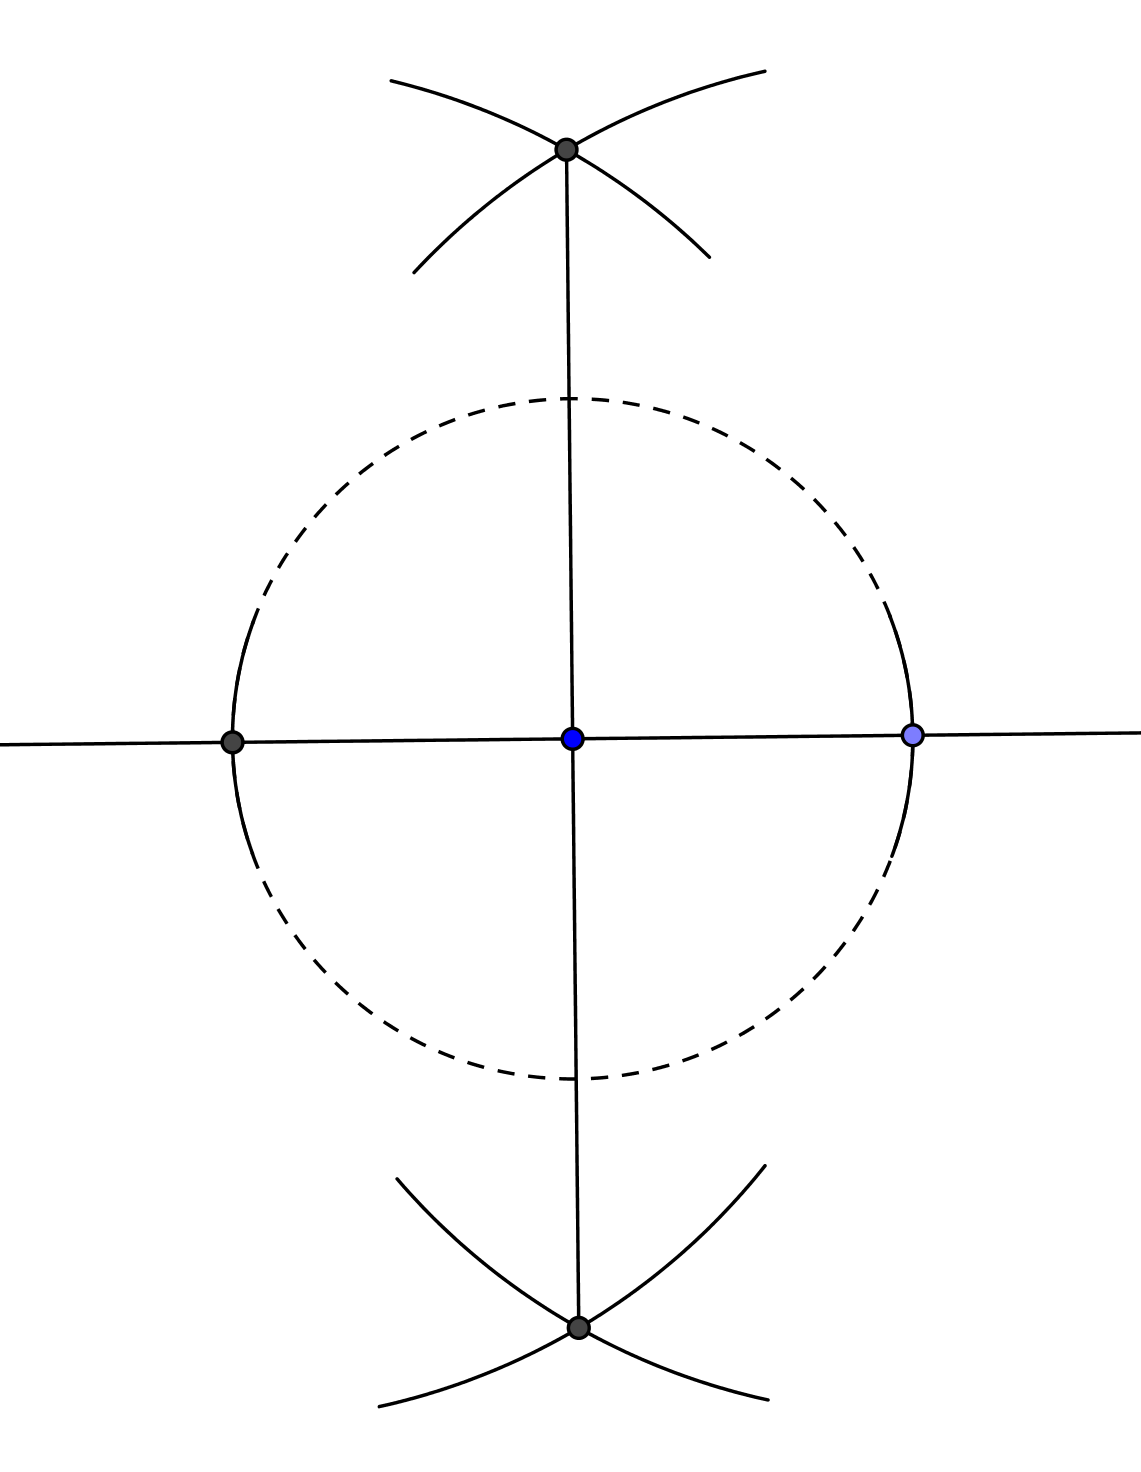
\includegraphics{perpOnLine.png}
\end{image}
\end{hint}
\end{freeResponse}
\end{problem}

\begin{problem}
Use a compass and straightedge to bisect a given angle. Explain the steps in your construction and how you know it works.
\begin{freeResponse}
\begin{hint}%[Bisecting an Angle]\index{compass and straightedge!bisecting an angle} 
%We wish to divide an angle in half.
\begin{enumerate}
\item Draw a circle with its center being the vertex of the 
angle.
%\item Draw a line segment where the circle intersects the lines.
%\item Bisect the new line segment.  The bisector will bisect the angle.
\item At each of the points where that circle intersects the sides of the angle, draw a circle with the same radius.
\item The two circles intersect in two points.  Draw a ray from the vertex of the angle through one of those points.  
\item The line bisects the angle.  
\end{enumerate}
\begin{image}

\includegraphics{bisectangle2.png}
\end{image}
\end{hint}
\end{freeResponse}
\end{problem}



\begin{problem}
Given an angle and some point [or a ray], use a compass and straightedge to copy the angle so that the new angle has as its vertex the given point [or a ray as one side of the angle]. Explain the steps in your construction and how you know it works.
\begin{freeResponse}
\begin{hint}%[Copying an Angle]\index{compass and straightedge!copying an angle} 
%Given a point on a line and some angle, we wish to copy the 
%given angle so that the new angle has the point as its 
%vertex and the line as one of its edges.
\begin{enumerate}
\item Open the compass to a fixed width and make a circle 
centered at the vertex of the angle.
\item Make a circle of the same radius on the line with the point [or on the ray].
\item Open the compass so that one end touches the first circle 
where it hits one side of the original angle, with the other end of the compass extended to where the first circle hits the other side of the original angle.
\item Draw a circle with the radius found above with its center 
where the second circle hits the line.
\item Connect the point to where the circles meet. This is the other side of the angle we are constructing.
\end{enumerate}
\begin{image}
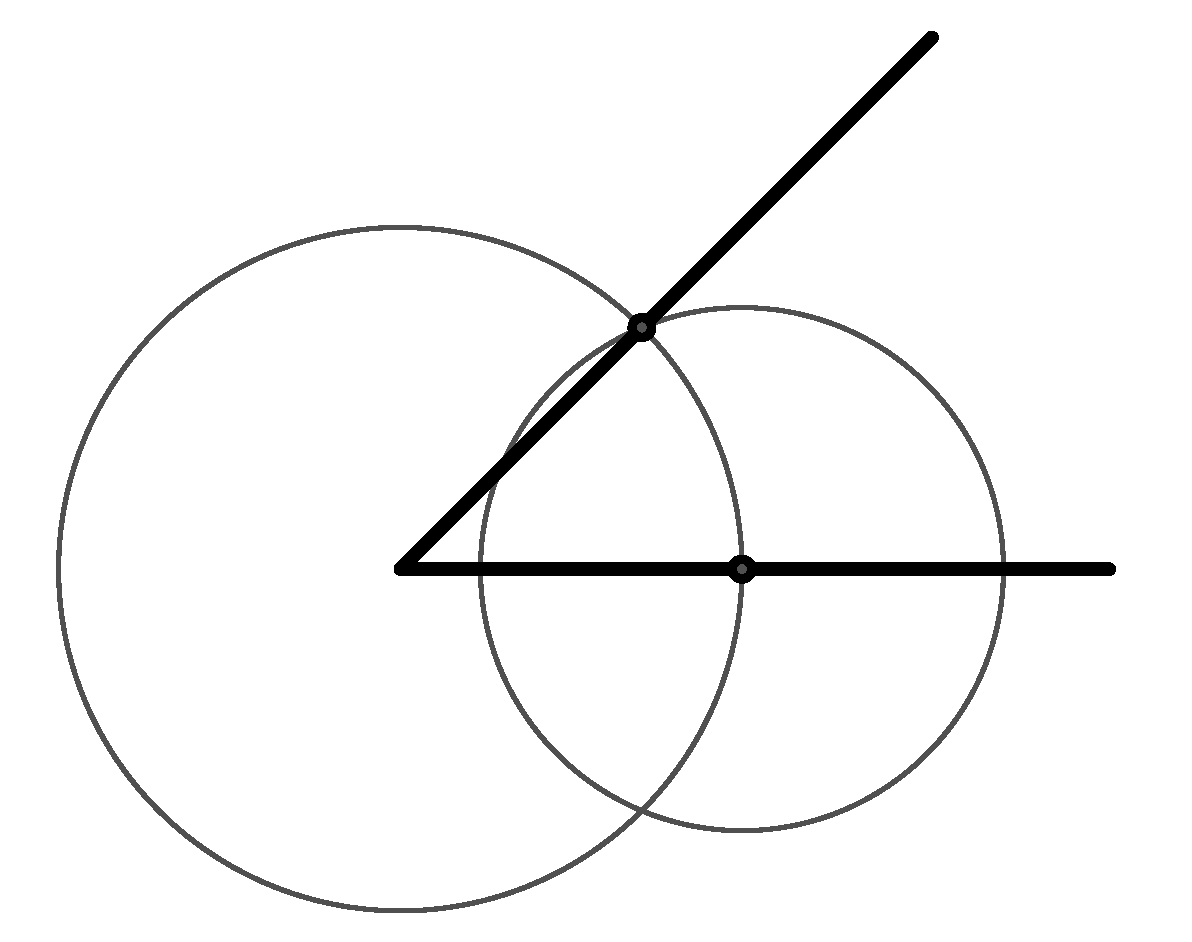
\includegraphics{copyangle.png}
\end{image}
\end{hint}
\end{freeResponse}
\end{problem}



\begin{problem}
Given a point and line, construct a line perpendicular to the given line that passes through the given point. Explain the steps in your construction and how you know it works.
\begin{freeResponse}
\begin{hint}%[Perpendicular to a Line through a Point]\index{compass and straightedge!perpendicular to a line through a point}  
%Given a point and a line, we wish to construct a line perpendicular to
the original line that passes through the given point.
\begin{enumerate}
\item Draw a circle centered at the point large enough  
       to intersect the line in two distinct points.
\item Bisect the line segment. The line used to do this 
       will be the desired line.
\end{enumerate}
\begin{image}
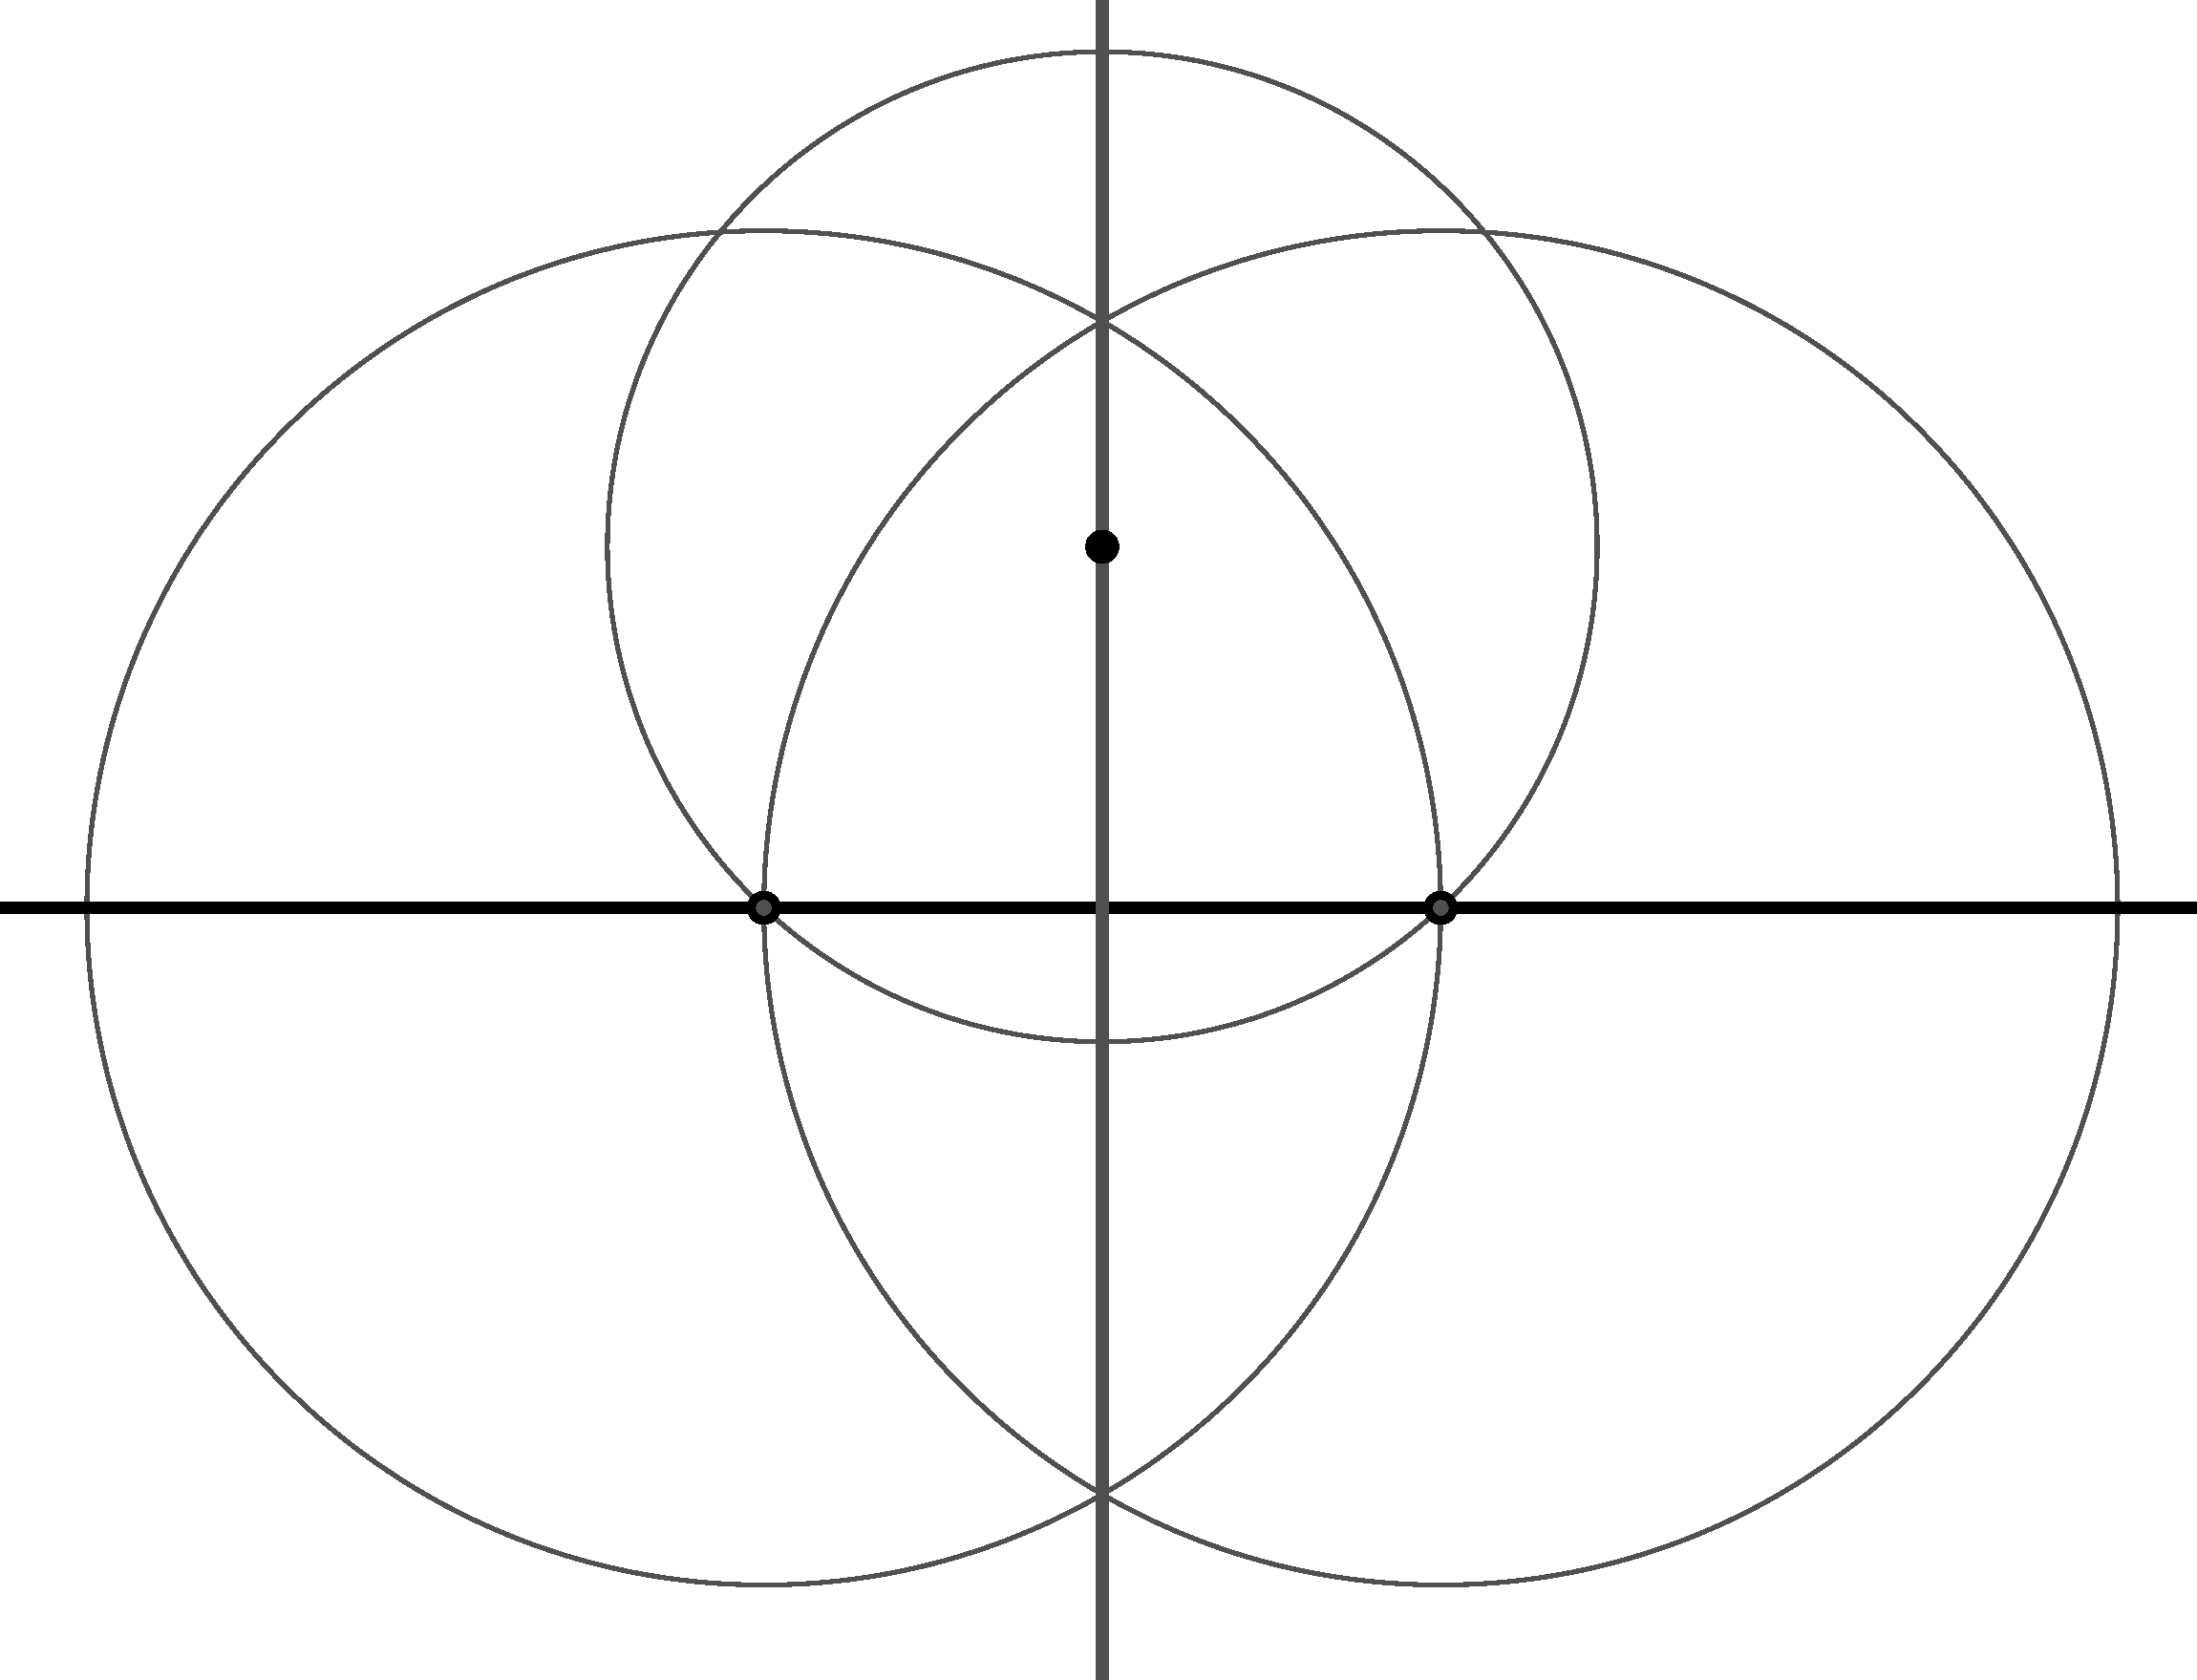
\includegraphics{perpfrompoint.png}
\end{image}
\end{hint}
\end{freeResponse}
\end{problem}

\begin{problem}
Given a point and line, construct a line parallel to the given line that passes through the given point. Explain the steps in your construction and how you know it works.
\begin{freeResponse}
\begin{hint}
Through the given point, construct a perpendicular to the given line.  Then through the same point, construct a perpendicular to the new line. 
\end{hint}
\end{freeResponse}
\end{problem}

%\begin{hint}%[Parallel to a Line through a Point]\index{compass and straightedge!parallel to a line through a point} 
% Given a line and a point, we wish to construct another line parallel
% to the first that passes through the given point.
%\begin{enumerate}
%\item Draw a circle centered at the given point and passing through the given line at two points.
%\item We now have an isosceles triangle, duplicate this triangle.
%\item Connect the top vertexes of the triangles and we get a parallel line.
%\end{enumerate}
%\begin{image}
%\includegraphics{parallel.pdf}
%\end{image}
%\end{hint}


\begin{problem}
Construct a $30$-$60$-$90$ right triangle. Explain the steps in your
  construction and how you know it works.
\begin{freeResponse}
\begin{hint}
Construct an equilateral triangle and cut it in half.  
\end{hint}
\end{freeResponse}
\end{problem}

\begin{problem}
Construct an isosceles right triangle. Explain the steps in your
  construction and how you know it works.
\begin{freeResponse}
\begin{hint}
Construct a square and draw a diagonal.  
\end{hint}
\end{freeResponse}
\end{problem}



\end{document}
